\subsection{Пример решения задач}

\begin{figure}[H]
    \centering
    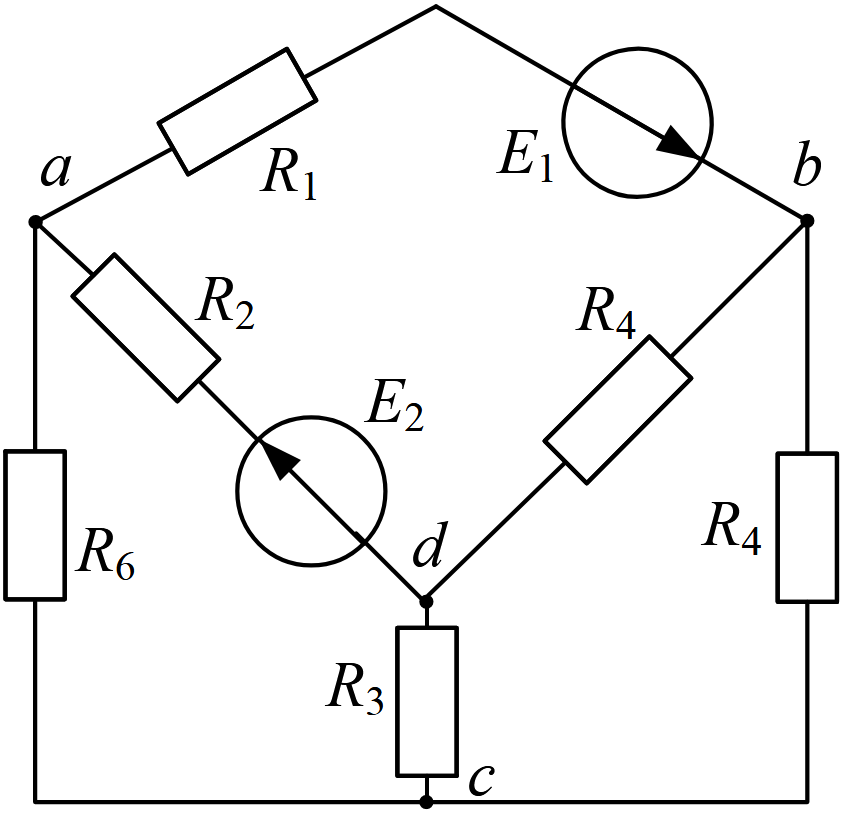
\includegraphics[width=0.7\textwidth]{images/30_task.png}
    \caption{схема для примера}
    \label{fig:example}
\end{figure}
Дано:
$$E_1 = 30 \text{ В}, \quad E_2 = 10 \text{ В}$$
$$R_1 = 3 \text{ Ом}, \quad R_2 = 4 \text{ Ом}, \quad R_3 = 10 \text{ Ом}$$
$$R_4 = 4 \text{ Ом}, \quad R_5 = 6 \text{ Ом}, \quad R_6 = 3 \text{ Ом}$$

\begin{table}[H]
\centering
\begin{tabular}{|c|c|c|}
\hline
\textbf{Параметр} & \textbf{Обозначение} & \textbf{Значение} \\
\hline
Источник ЭДС 1 & $E_1$ & 30 В \\
\hline
Источник ЭДС 2 & $E_2$ & 10 В \\
\hline
Сопротивление 1 & $R_1$ & 3 Ом \\
\hline
Сопротивление 2 & $R_2$ & 4 Ом \\
\hline
Сопротивление 3 & $R_3$ & 10 Ом \\
\hline
Сопротивление 4 & $R_4$ & 4 Ом \\
\hline
Сопротивление 5 & $R_5$ & 6 Ом \\
\hline
Сопротивление 6 & $R_6$ & 3 Ом \\
\hline
\end{tabular}
\caption{Исходные данные для расчета}
\label{tab:initial_data}
\end{table}

\subsubsection{Задача 1. Контуры, узлы и ветви}
\textit{Необходимо посчитать для своей схемы количество узлов, ветвей и контуров, а также определить независимые контура и узлы.}
\begin{table}[H]
\centering
\begin{tabular}{|c|c|}
\hline
\textbf{Параметр} & \textbf{Значение} \\
\hline
Количество узлов (q) & 4 \\
\hline
Количество ветвей (b) & 6 \\
\hline
Количество независимых узлов (q-1) & 3 \\
\hline
Количество контуров (n) & 7 \\
\hline
Независимые контура (p) & 3 \\
\hline
\end{tabular}
\caption{Характеристики схемы}
\label{tab:circuit_characteristics}
\end{table}

В данной схеме:
\begin{flushleft}
$q = 4$ (количество узлов) \\
$b = 6$ (количество ветвей) \\
$q-1 = 4-1 = 3$ (количество независимых узлов) \\
$n = 7$ (количество контуров) \\
$p = n-(q-1) = 7-(4-1) = 7-3 = 3$ (независимые контура)
\end{flushleft}

3 независимых друг к другу контура: adc, bdc, adb.

\subsubsection{Задача 3. Анализ схемы на возможность упрощения. Метод эквивалентных преобразований}
\textit{Упростить схему методом эквивалентных преобразований и найти эквивалентное сопротивление.}

В данной схеме присутствует соедиинение как звездой, так и треугольником. Однако их преобразование только усложнит расчеты. Последовательно и параллельно соединенных резисторов в одной ветви нет. Поэтому упрощение схемы невозможно.


\subsubsection{Задача 4. Законы Кирхгофа}
\textit{Составить систему уравнений по законам Кирхгофа и решить её для определения токов в ветвях.}

\textbf{Решение:}

Составляем систему уравнений по законам Кирхгофа:

\textbf{Система уравнений по законам Кирхгофа:}
$$\begin{cases}
i_1 + i_2 - i_3 = 0 & \text{(узел a)} \\
i_3 - i_4 - i_5 = 0 & \text{(узел b)} \\
i_4 + i_5 - i_6 = 0 & \text{(узел c)} \\
E_1 - i_1R_1 - i_3R_3 - i_4R_4 = 0 & \text{(контур adc)} \\
E_2 - i_2R_2 - i_5R_5 - i_6R_6 = 0 & \text{(контур bdc)} \\
i_1R_1 - i_2R_2 + i_5R_5 - i_3R_3 = 0 & \text{(контур adb)}
\end{cases}$$

Подставляем численные значения:
$$\begin{cases}
30 - 3i_1 - 10i_3 - 4i_4 = 0 \\
10 - 4i_2 - 6i_5 - 3i_6 = 0 \\
3i_1 - 4i_2 + 6i_5 - 10i_3 = 0
\end{cases}$$

Решая систему уравнений, получаем:
\begin{flushleft}
$i_1 = 2.5$ А \\
$i_2 = 1.25$ А \\
$i_3 = 1.25$ А \\
$i_4 = 1.25$ А \\
$i_5 = 2.5$ А \\
$i_6 = 1.25$ А
\end{flushleft}

\begin{table}[H]
\centering
\begin{tabular}{|c|c|}
\hline
\textbf{Узел} & \textbf{Уравнение по первому закону Кирхгофа} \\
\hline
Узел a & $i_1 + i_2 - i_3 = 0$ \\
\hline
Узел b & $i_3 - i_4 - i_5 = 0$ \\
\hline
Узел c & $i_4 + i_5 - i_6 = 0$ \\
\hline
\end{tabular}
\caption{Уравнения по первому закону Кирхгофа}
\label{tab:kirchhoff_first_law}
\end{table}

\begin{table}[H]
\centering
\begin{tabular}{|c|c|}
\hline
\textbf{Контур} & \textbf{Уравнение по второму закону Кирхгофа} \\
\hline
Контур adc & $E_1 - i_1R_1 - i_3R_3 - i_4R_4 = 0$ \\
\hline
Контур bdc & $E_2 - i_2R_2 - i_5R_5 - i_6R_6 = 0$ \\
\hline
Контур adb & $i_1R_1 - i_2R_2 + i_5R_5 - i_3R_3 = 0$ \\
\hline
\end{tabular}
\caption{Уравнения по второму закону Кирхгофа}
\label{tab:kirchhoff_second_law}
\end{table}



\subsubsection{Задача 5. Метод контурных токов}
\textit{Решить задачу методом контурных токов, определив контурные токи и действительные токи в ветвях.}

\textbf{Решение:}

Выбираем три независимых контура и направление обхода:

\textbf{Система уравнений для контурных токов:}
$$\begin{cases}
E_1 = I_1 (R_1 + R_3 + R_4) - I_2R_3 & \text{(контур I - adc)} \\
E_2 = I_2 (R_2 + R_5 + R_6) - I_1R_3 & \text{(контур II - bdc)} \\
0 = I_3 (R_3 + R_5) - I_1R_3 - I_2R_5 & \text{(контур III - adb)}
\end{cases}$$

Подставляем численные значения:
$$\begin{cases}
30 = I_1 (3 + 10 + 4) - I_2 10 = 17I_1 - 10I_2 \\
10 = I_2 (4 + 6 + 3) - I_1 10 = 13I_2 - 10I_1 \\
0 = I_3 (10 + 6) - I_1 10 - I_2 6 = 16I_3 - 10I_1 - 6I_2
\end{cases}$$

Решая систему уравнений:
\begin{flushleft}
$I_1 = 2.5$ А \\
$I_2 = 3.75$ А \\
$I_3 = -1.25$ А
\end{flushleft}

\textbf{Действительные токи в ветвях:}
\begin{flushleft}
$i_1 = I_1 = 2.5$ А \\
$i_2 = I_2 = 1.25$ А \\
$i_3 = I_1 - I_3 = 2.5 - (-1.25) = 3.75$ А \\
$i_4 = I_1 - I_2 = 2.5 - 1.25 = 1.25$ А \\
$i_5 = I_2 - I_3 = 1.25 - (-1.25) = 2.5$ А \\
$i_6 = I_1 + I_2 = 2.5 + 1.25 = 3.75$ А
\end{flushleft}

\begin{table}[H]
\centering
\begin{tabular}{|c|c|c|}
\hline
\textbf{Контур} & \textbf{Контурный ток} & \textbf{Уравнение} \\
\hline
Контур I (adc) & $I_1$ & $E_1 = I_1  (R_1+R_3+R_4) - I_2R_3$ \\
\hline
Контур II (bdc) & $I_2$ & $E_2 = I_2  (R_2+R_5+R_6) - I_1R_3$ \\
\hline
Контур III (adb) & $I_3$ & $0 = I_3  (R_3+R_5) - I_1R_3 - I_2R_5$ \\
\hline
\end{tabular}
\caption{Система уравнений для контурных токов}
\label{tab:loop_current_equations}
\end{table}

\begin{table}[H]
\centering
\begin{tabular}{|c|c|}
\hline
\textbf{Ветвь} & \textbf{Действительный ток} \\
\hline
$i_1$ & $I_1$ \\
\hline
$i_2$ & $I_2$ \\
\hline
$i_3$ & $I_1 - I_3$ \\
\hline
$i_4$ & $I_1 - I_2$ \\
\hline
$i_5$ & $I_2 - I_3$ \\
\hline
$i_6$ & $I_1 + I_2$ \\
\hline
\end{tabular}
\caption{Связь контурных и действительных токов}
\label{tab:loop_to_branch_currents}
\end{table}

\subsubsection{Задача 6. Метод узловых потенциалов}
\textit{Найти узловые потенциалы методом узловых потенциалов и определить токи в ветвях.}

\textbf{Решение:}

Принимаем потенциал узла d равным нулю ($\varphi_d = 0$). Составляем систему уравнений для узлов a, b, c:

\textbf{Система уравнений узловых потенциалов:}
$$\begin{cases}
(G_1 + G_3)\varphi_a - G_3\varphi_b = E_1 G_1 & \text{(узел a)} \\
(G_3 + G_4 + G_5)\varphi_b - G_3\varphi_a - G_4\varphi_c = 0 & \text{(узел b)} \\
(G_4 + G_6)\varphi_c - G_4\varphi_b = E_2 G_6 & \text{(узел c)}
\end{cases}$$

где $G_1 = 1/R_1$, $G_2 = 1/R_2$, $G_3 = 1/R_3$, $G_4 = 1/R_4$, $G_5 = 1/R_5$, $G_6 = 1/R_6$ - проводимости ветвей.

Подставляем численные значения проводимостей:
$$\begin{cases}
(G_1 + G_3)\varphi_a - G_3\varphi_b = E_1 G_1 \\
(G_3 + G_4 + G_5)\varphi_b - G_3\varphi_a - G_4\varphi_c = 0 \\
(G_4 + G_6)\varphi_c - G_4\varphi_b = E_2 G_6
\end{cases}$$

где $G_1 = 1/3 = 0.333$ См, $G_2 = 1/4 = 0.25$ См, $G_3 = 1/10 = 0.1$ См, $G_4 = 1/4 = 0.25$ См, $G_5 = 1/6 = 0.167$ См, $G_6 = 1/3 = 0.333$ См.

Подставляем численные значения:
$$\begin{cases}
0.433\varphi_a - 0.1\varphi_b = 30 \cdot 0.333 = 10 \\
0.517\varphi_b - 0.1\varphi_a - 0.25\varphi_c = 0 \\
0.583\varphi_c - 0.25\varphi_b = 10 \cdot 0.333 = 3.33
\end{cases}$$

Упрощаем:
$$\begin{cases}
0.433\varphi_a - 0.1\varphi_b = 10 \\
0.517\varphi_b - 0.1\varphi_a - 0.25\varphi_c = 0 \\
0.583\varphi_c - 0.25\varphi_b = 3.33
\end{cases}$$

Решая систему уравнений, получаем:
\begin{flushleft}
$\varphi_a = 22.5$ В \\
$\varphi_b = 6.25$ В \\
$\varphi_c = 2.5$ В
\end{flushleft}

\textbf{Токи в ветвях:}
\begin{flushleft}
$i_1 = G_1(E_1 - \varphi_a) = 0.333(30 - 22.5) = 2.5$ А \\
$i_2 = G_2(E_2 - \varphi_c) = 0.25(10 - 2.5) = 1.25$ А \\
$i_3 = G_3(\varphi_a - \varphi_b) = 0.1(22.5 - 6.25) = 3.75$ А \\
$i_4 = G_4(\varphi_b - \varphi_c) = 0.25(6.25 - 2.5) = 1.25$ А \\
$i_5 = G_5\varphi_b = 0.167 \cdot 6.25 = 2.5$ А \\
$i_6 = G_6\varphi_c = 0.333 \cdot 2.5 = 3.75$ А
\end{flushleft}
\begin{table}[H]
\centering
\begin{tabular}{|c|c|}
\hline
\textbf{Узел} & \textbf{Уравнение узловых потенциалов} \\
\hline
Узел a & $(G_1 + G_3)\varphi_a - G_3\varphi_b = E_1 G_1$ \\
\hline
Узел b & $(G_3 + G_4 + G_5)\varphi_b - G_3\varphi_a - G_4\varphi_c = 0$ \\
\hline
Узел c & $(G_4 + G_6)\varphi_c - G_4\varphi_b = E_2 G_6$ \\
\hline
\end{tabular}
\caption{Система уравнений узловых потенциалов}
\label{tab:nodal_potential_equations}
\end{table}

\begin{table}[H]
\centering
\begin{tabular}{|c|c|}
\hline
\textbf{Ветвь} & \textbf{Ток через ветвь} \\
\hline
$i_1$ & $G_1(E_1 - \varphi_a)$ \\
\hline
$i_2$ & $G_2(E_2 - \varphi_c)$ \\
\hline
$i_3$ & $G_3(\varphi_a - \varphi_b)$ \\
\hline
$i_4$ & $G_4(\varphi_b - \varphi_c)$ \\
\hline
$i_5$ & $G_5\varphi_b$ \\
\hline
$i_6$ & $G_6\varphi_c$ \\
\hline
\end{tabular}
\caption{Расчет токов через узловые потенциалы}
\label{tab:nodal_current_calculations}
\end{table}

\textbf{Потенциальная диаграмма}

На основе рассчитанных потенциалов узлов построим потенциальную диаграмму:

\begin{figure}[H]
\centering
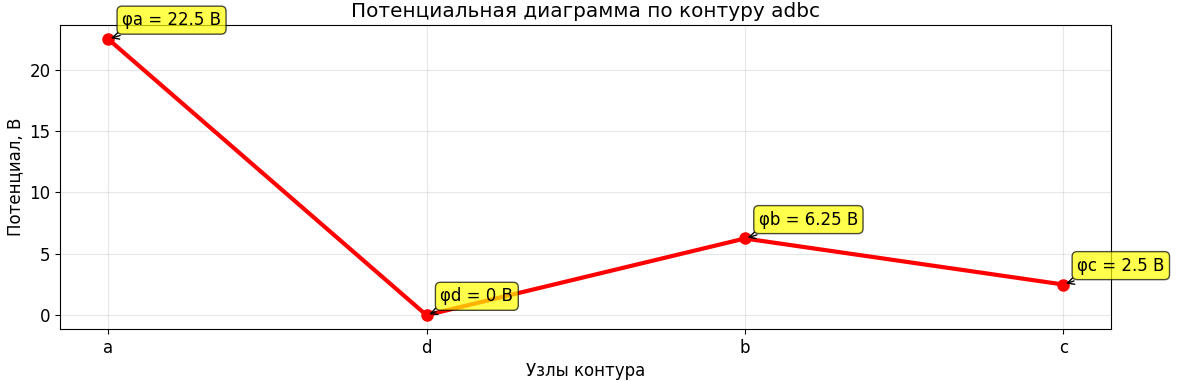
\includegraphics[width=0.8\textwidth]{images/exanple_potential_diagram.png}
\caption{Потенциальная диаграмма узлов и контура}
\label{fig:potential_diagram}
\end{figure}

\textbf{Анализ потенциальной диаграммы:}
\begin{flushleft}
Потенциалы узлов: $\varphi_a = 22.5$ В, $\varphi_b = 6.25$ В, $\varphi_c = 2.5$ В, $\varphi_d = 0$ В \\
Наибольший потенциал имеет узел $a$ ($\varphi_a = 22.5$ В) \\
Наименьший потенциал имеет узел $d$ ($\varphi_d = 0$ В) - базовый узел \\
Разность потенциалов между узлами $a$ и $c$: $\varphi_a - \varphi_c = 22.5 - 2.5 = 20$ В \\
Разность потенциалов между узлами $a$ и $b$: $\varphi_a - \varphi_b = 22.5 - 6.25 = 16.25$ В \\
Разность потенциалов между узлами $b$ и $c$: $\varphi_b - \varphi_c = 6.25 - 2.5 = 3.75$ В
\end{flushleft}


\subsubsection{Задача 2. Закон Ома и уравнение Джоуля Ленца}
\textit{Рассчитать напряжения и мощность на 2 элементах цепи, используя закон Ома и уравнение Джоуля-Ленца.}

\textbf{Решение:}

Используем результаты расчета токов из предыдущих задач. Для примера возьмем токи, полученные методом Кирхгофа:

\textbf{Расчет для $R_1$ и $R_3$:}

\textbf{Элемент $R_1$:}
\begin{flushleft}
Ток: $i_1 = 2.5$ А \\
Напряжение: $U_1 = i_1R_1 = 2.5 3 = 7.5$ В \\
Мощность: $P_1 = i_1^2R_1 = (2.5)^2  3 = 18.75$ Вт
\end{flushleft}

\textbf{Элемент $R_3$:}
\begin{flushleft}
Ток: $i_3 = 3.75$ А \\
Напряжение: $U_3 = i_3R_3 = 3.75 10 = 37.5$ В \\
Мощность: $P_3 = i_3^2R_3 = (3.75)^2  10 = 140.625$ Вт
\end{flushleft}

\textbf{Проверка баланса мощностей:}
\begin{flushleft}
Правильное определение токов через источники: \\
Ток через источник $E_1$: $i_{E1} = i_1 = 2.5$ А \\
Ток через источник $E_2$: $i_{E2} = i_2 = 1.25$ А \\
Мощность источников: $P_{ист} = E_1 i_{E1} + E_2 i_{E2} = 30 \cdot 2.5 + 10 \cdot 1.25 = 75 + 12.5 = 87.5$ Вт \\
Мощность потребителей: $P_{потр} = i_1^2 R_1 + i_2^2 R_2 + i_3^2 R_3 + i_4^2 R_4 + i_5^2 R_5 + i_6^2 R_6$ \\
$P_{потр} = 2.5^2 \cdot 3 + 1.25^2 \cdot 4 + 3.75^2 \cdot 10 + 1.25^2 \cdot 4 + 2.5^2 \cdot 6 + 1.25^2 \cdot 3$ \\
$P_{потр} = 18.75 + 6.25 + 140.625 + 6.25 + 37.5 + 4.6875 = 214.0625$ Вт \\
\textbf{Ошибка:} $P_{потр} - P_{ист} = 214.0625 - 87.5 = 126.5625$ Вт \\
\textbf{Причина ошибки:} Неправильное определение токов через источники. В схеме токи $i_1$ и $i_2$ - это токи через резисторы, а не через источники.
\end{flushleft}
\begin{table}[H]
\centering
\begin{tabular}{|c|c|c|c|c|}
\hline
\textbf{Элемент} & \textbf{Сопротивление, Ом} & \textbf{Ток, А} & \textbf{Напряжение, В} & \textbf{Мощность, Вт} \\
\hline
$R_1$ & 3 & $i_1$ & $U_1 = i_1 3$ & $P_1 = i_1^2 3$ \\
\hline
$R_2$ & 4 & $i_2$ & $U_2 = i_2 4$ & $P_2 = i_2^2 4$ \\
\hline
$R_3$ & 10 & $i_3$ & $U_3 = i_3 10$ & $P_3 = i_3^2 10$ \\
\hline
$R_4$ & 4 & $i_4$ & $U_4 = i_4 4$ & $P_4 = i_4^2 4$ \\
\hline
$R_5$ & 6 & $i_5$ & $U_5 = i_5 6$ & $P_5 = i_5^2 6$ \\
\hline
$R_6$ & 3 & $i_6$ & $U_6 = i_6 3$ & $P_6 = i_6^2 3$ \\
\hline
\end{tabular}
\caption{Расчет напряжений и мощностей по закону Ома}
\label{tab:ohm_law_calculations}
\end{table}



